% Standalone supplementary build; the main paper and its legacy protocol fragment
% remain unchanged. Compile from the repository root with pdfLaTeX/latexmk.
\documentclass[10pt,twocolumn,letterpaper]{article}
\usepackage[review]{cvpr}
%% This file contains a number of tweaks that are typically applied to the main document.
%% They are not enabled by default, but can be enabled by uncommenting the relevant lines.


%%
%% Official support for 2-column teaser figure
%%
\usepackage{cuted} %< for strip environment

%%
%% For auto-referencing of figures (see fig/teaser.tex and \label{} therein) 
%%
\usepackage{currfile} %< for \currfilebase macro

%%
%% caption and (global) spacing overrides
%%
\usepackage{caption} %< for "\captionof" commands (teaser)
% \setlength{\abovecaptionskip}{.5em} % space above caption
% \setlength{\belowcaptionskip}{1em} % space below caption

%%
%% Inline annotations; for predefined colors, refer to "dvipsnames" in the xcolor package:
%% https://tinyurl.com/overleaf-colors
%%
\newcommand{\red}[1]{{\color{red}#1}}
\newcommand{\todo}[1]{{\color{red}#1}}
\newcommand{\TODO}[1]{\textbf{\color{red}[TODO: #1]}}
%%
%% Disable for camera ready / submission by uncommenting these lines:
%%
% \renewcommand{\TODO}[1]{}
% \renewcommand{\todo}[1]{#1}

%%
%% Work harder in optimizing text layout. Typically shrinks text by 1/6 of page, enable
%% it at the very end of the writing process, when you are just above the page limit.
%%
% \usepackage{microtype}

%%
%% Fine-tune paragraph spacing.
%%
% \renewcommand{\paragraph}[1]{\vspace{.5em}\noindent\textbf{#1.}}

%%
%% Globally adjusts space between figure and caption.
%%
% \setlength{\abovecaptionskip}{.5em}

%%
%% Allows "the use of \paper to refer to the project name"
%% with automatic management of space at the end of the word.
%%
% \usepackage{xspace}
% \newcommand{\paper}{ProjectName\xspace}

%%
%% Commonly used math definitions.
%%
% \DeclareMathOperator*{\argmin}{arg\,min}
% \DeclareMathOperator*{\argmax}{arg\,max}

%%
%% Tighten underline.
%%
% \usepackage{soul}
% \setuldepth{foobar}

%%
%% Reconfigure paragraph (tweaks spacing)
%%

% graphicx, amsmath, and booktabs are already provided by cvpr.sty.
\usepackage{tabularx}
\usepackage{algpseudocode}
% Normal float gaps for the standalone supplement.
\setlength{\textfloatsep}{6pt plus 2pt minus 2pt}
\setlength{\dbltextfloatsep}{6pt plus 2pt minus 2pt}
\setlength{\floatsep}{6pt plus 2pt minus 2pt}
\setlength{\dblfloatsep}{6pt plus 2pt minus 2pt}
\setlength{\intextsep}{6pt plus 2pt minus 2pt}
\definecolor{cvprblue}{rgb}{0.21,0.49,0.74}
\usepackage[pagebackref,breaklinks,colorlinks,allcolors=cvprblue]{hyperref}
\hypersetup{pdfauthor={},pdftitle={Supplementary Material}}
\def\confName{CVPR}
\def\confYear{2027}
\title{Fixing the Score Is Not Fixing the Order:\\
Ordinal Transfer to Unseen Grades in Adapted CLIP\\[0.3em]
{\large Supplementary Material}}
\author{Anonymous Authors}

\begin{document}
\maketitle
\appendix
\renewcommand{\thefigure}{S\arabic{figure}}
\renewcommand{\thetable}{S\arabic{table}}
\renewcommand{\theequation}{S\arabic{equation}}
% Navigation: unnumbered; does not consume the appendix letter A.
\section*{Guide to the Supplement}
Sections A--B examine the two central design choices: the strength of adaptation and the source of a missing grade's displacement.
The remaining sections establish how transfer depends on supervision, extend the evaluation, and provide the derivations and protocols.

\noindent\begin{tabularx}{\columnwidth}{@{}lX@{}}
\textbf{A} & Global blending and classification trade-offs.\\
\textbf{B} & Reference preservation and displacement inheritance.\\
\textbf{C} & Grade support, missing patterns, and full support.\\
\textbf{D} & Adaptation regimes, backbones, and domains.\\
\textbf{E} & Derivations and the inference algorithm.\\
\textbf{F} & Configurations, prompts, and evaluation protocols.
\end{tabularx}

\noindent The central comparisons are in Secs.~\ref{sec:supp_best_blend}--\ref{sec:supp_error_tradeoffs} and \ref{sec:supp_keep_inherit}; Sec.~\ref{sec:supp_inheritance_error} explains the remaining inheritance error.

\section{Beyond Global Blending}
\label{sec:supp_blending}

TIE changes the source of a missing grade's adaptation; global blending changes its strength.
We examine this distinction across adapter configurations and at the best evaluated blending strength, then compare the resulting classification trade-offs.

\subsection{Configuration-Level Ranking Curves}
\label{sec:supp_config_curves}

Let $T$ and $S$ denote the zero-shot and adapted scores, and let $D=S-T$.
Global score blending provides an output-space counterpart to zero-shot/fine-tuned weight interpolation~\cite{wortsman2022robust}.
At strength $\lambda$, the two score constructions are
\begin{equation}
\begin{aligned}
 B_\lambda &= T+\lambda D,\\
 S^{\mathrm{TIE}}_\lambda &= T+\lambda\mathcal L_{\mathcal U}(D).
\end{aligned}
\label{eq:supp_matched_paths}
\end{equation}
Here $\mathcal U$ is the set of missing grades and $\mathcal L_{\mathcal U}$ is the inheritance operator from the main paper.
At every matched strength, the two constructions have identical seen-grade scores and differ only in the missing grades' displacement.
Class-bias calibration preserves their respective pairwise rankings by Proposition~1 of the main paper.

Sections~A.1--A.2 use the three interior missing-grade masks and three seeds for each of the nine adapter configurations.
Each configuration curve therefore averages nine conditions; the dataset mean averages all nine configurations equally, for 81 conditions per dataset.
We evaluate $\lambda\in\{0,0.1,\ldots,1.5,2.0\}$.
The zero-shot reference is recovered at $\lambda=0$, $\lambda=1$ retains the original adaptation strength, and $\lambda>1$ extrapolates.
MS-AUC averages pair AUROC over adjacent missing--seen grade pairs.

Figure~\ref{fig:supp_config_curves} resolves the difference between the two paths by configuration.
At $\lambda=1$, TIE improves MS-AUC in 35 of the 36 configuration--dataset settings: eight of nine on Adience and all nine on HCI, FairFace, and KonIQ.
This is the interior-mask counterpart of the 34/36 result over all six masks in the main paper.
The improvement spans the adaptation configurations, while the curves expose differences in its magnitude and dependence on strength.

\begin{figure*}[!t]
\centering
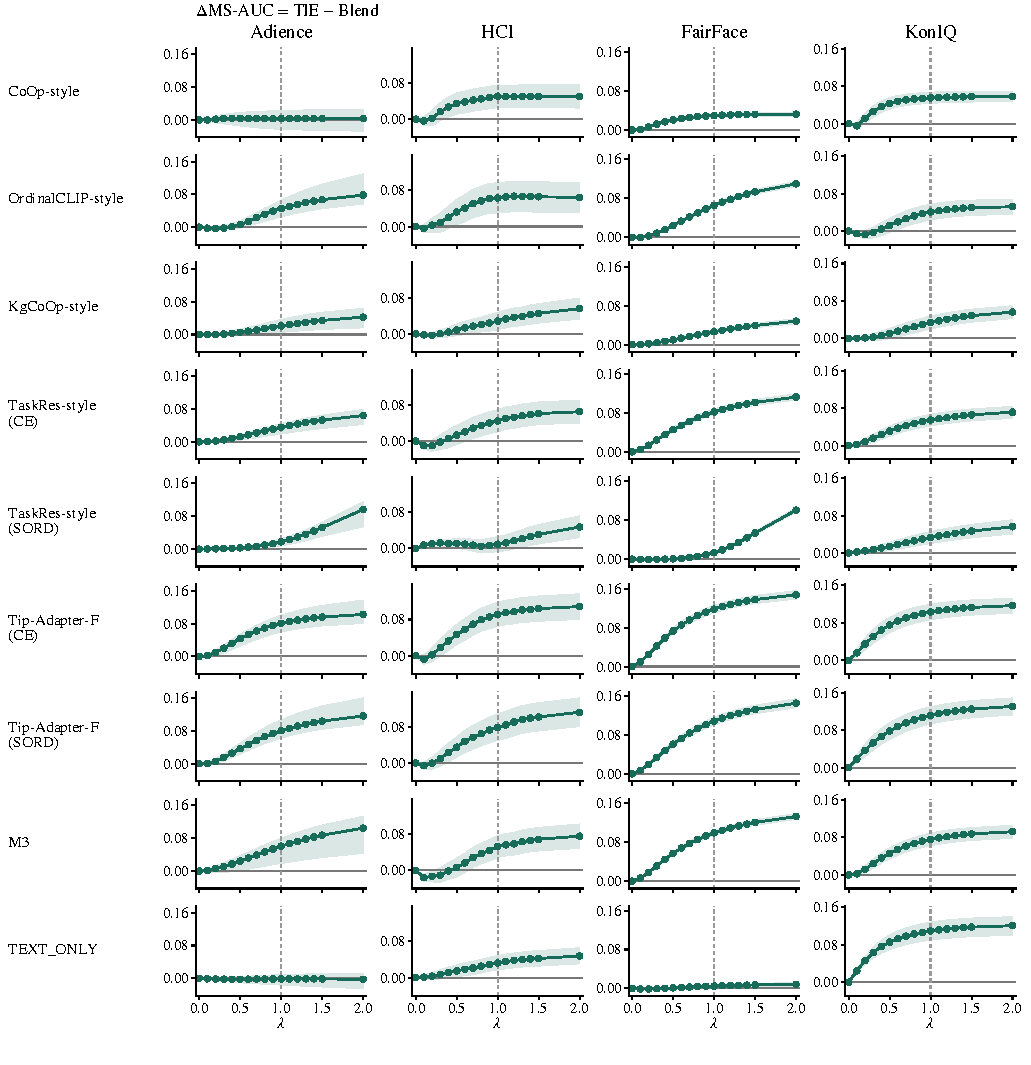
\includegraphics[width=\textwidth]{figures/supp/supp_a_configuration_curves.pdf}
\caption{\textbf{Ranking gains across configurations and strengths.}
Each panel shows $\Delta=\text{MS-AUC}(\text{TIE})-\text{MS-AUC}(\text{Blend})$ for one configuration and dataset, averaged over three interior masks and three seeds.
Points mark all 17 evaluated strengths; available paired pointwise 95\% bootstrap intervals are shaded.
Horizontal lines mark zero gain and vertical dashed lines mark $\lambda=1$.
All panels in a column share their vertical scale.
Configuration definitions are given in Sec.~F.2.}
\label{fig:supp_config_curves}
\end{figure*}

\subsection{Matched Strengths and the Best Evaluated Blend}
\label{sec:supp_best_blend}

At the original adaptation strength, TIE gains 0.038--0.069 MS-AUC over Blend (Table~\ref{tab:supp_best_blend}).
Across the grid, the paired 95\% interval is entirely positive at 59 of the 64 nonzero dataset--strength combinations: 14/16 on Adience, 13/16 on HCI, and 16/16 on both FairFace and KonIQ.
HCI at $\lambda=0.1$ is the only negative interval.
The intervals cross zero at $\lambda=0.1,0.2$ on Adience and $\lambda=0.2,0.3$ on HCI.

We next give Blend its best strength on the grid, chosen separately for each dataset using test MS-AUC and shared across all nine configurations.
TIE remains at $\lambda=1$.
On HCI, FairFace, and KonIQ, it exceeds even this best Blend by 0.042, 0.018, and 0.067, respectively.
TIE also exceeds the zero-shot reference on these three benchmarks by 0.113, 0.025, and 0.096.
Its gains therefore go beyond recovering the reference order.

\begin{table*}[t]
\centering
\caption{\textbf{Original-strength transfer versus the best global blend.}
Results use the interior masks and equal configuration weighting of the main paper's Fig.~2.
The confidence interval belongs to the paired difference at the fixed strength $\lambda=1$.
Best Blend maximizes dataset-mean test MS-AUC over the 17-point grid with one shared strength $\lambda^\star$; the final column reports TIE at $\lambda=1$ minus this best Blend.
Differences are computed before rounding.}
\label{tab:supp_best_blend}
\small
\begin{tabular*}{\textwidth}{@{\extracolsep{\fill}}lcccc@{}}
\toprule
Dataset & TIE$_1$ & TIE$_1$ $-$ Blend$_1$ [95\% CI]
 & Best Blend ($\lambda^\star$) & TIE$_1$ $-$ Best Blend\\
\midrule
Adience  & 0.906 & $+0.038\;[0.024,0.046]$ & 0.918 (0.1) & $-0.012$\\
HCI      & 0.742 & $+0.050\;[0.034,0.066]$ & 0.700 (0.5) & $\mathbf{+0.042}$\\
FairFace & 0.817 & $+0.061\;[0.058,0.064]$ & 0.800 (0.2) & $\mathbf{+0.018}$\\
KonIQ    & 0.635 & $+0.069\;[0.057,0.080]$ & 0.568 (0.6) & $\mathbf{+0.067}$\\
\bottomrule
\end{tabular*}
\end{table*}

Adience starts from a strong zero-shot ranking: 0.916 MS-AUC, compared with 0.867 after adaptation.
TIE at $\lambda=1$ reaches 0.906 and recovers 79\% of this loss.
From $\lambda=0$ to $2$, its MS-AUC decreases by 0.030, compared with 0.097 for Blend.
Here, transfer preserves much more of the reference ordering as adaptation strength increases.

\subsection{Missing--Seen Error Trade-offs}
\label{sec:supp_error_tradeoffs}

Figure~\ref{fig:supp_error_tradeoffs} places the six methods from Table~1 of the main paper in the plane of seen-grade and missing-grade MAE.
This comparison uses all six missing-grade masks, giving 162 conditions per dataset with equal weighting across configurations.
Within each condition, Missing MAE averages the per-grade errors over missing grades; Seen MAE averages errors over seen-grade test images.
Lower values on both axes are better.
The suffix +C denotes class-bias calibration.
Each calibrated method uses its own offset under the same seen-validation protocol.
Both Blend selectors use validation data; the test-set maximization in Sec.~A.2 serves only the ranking comparison.

\begin{figure*}[!t]
\centering
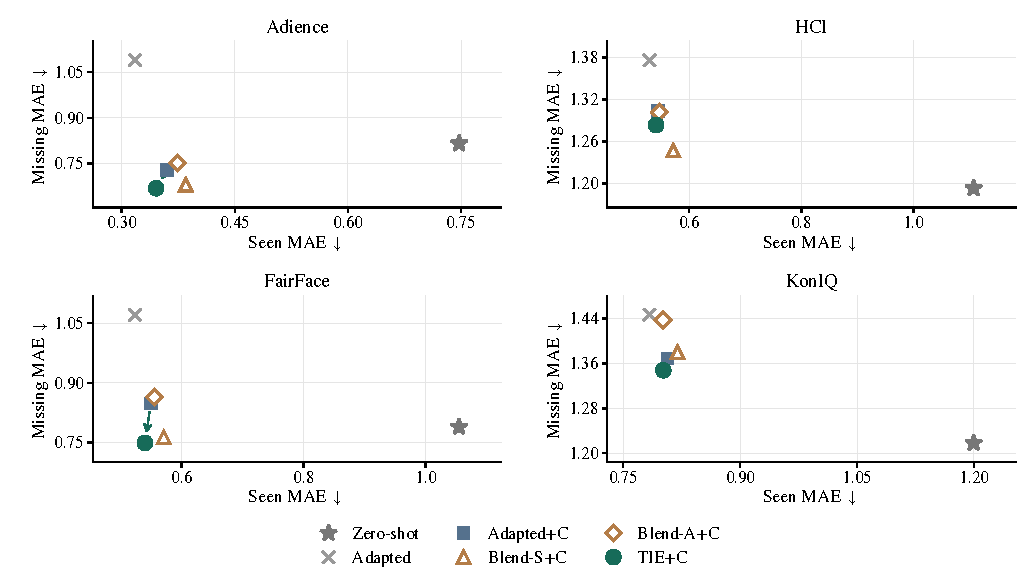
\includegraphics[width=\textwidth]{figures/supp/supp_a_error_tradeoff.pdf}
\caption{\textbf{Preserving adaptation while reducing missing-grade error.}
Each point is a method from Table~1 of the main paper, averaged over nine configurations, six masks, and three seeds.
Lower left is better.
Missing MAE is averaged across missing grades; Seen MAE is averaged across seen-grade images.
The green arrows connect Adapted+C to TIE+C.
The zero-shot point uses the reference scores for all grades.
Each dataset retains its own axis ranges.}
\label{fig:supp_error_tradeoffs}
\end{figure*}

TIE+C lowers both missing-grade and seen-grade MAE relative to Adapted+C on all four benchmarks.
Returning entirely to zero-shot produces a different trade-off.
On HCI, zero-shot has lower Missing MAE than TIE+C, 1.193 versus 1.284, but its Seen MAE is 1.108 versus 0.541.
KonIQ shows the same pattern: Missing MAE is 1.218 versus 1.348, while Seen MAE is 1.200 versus 0.802.
TIE retains the benefit of adaptation on seen grades while reducing the damage to missing grades.

HCI also exposes the trade-off between the calibrated methods.
Blend-S+C reaches lower Missing MAE than TIE+C, 1.247 versus 1.284, with higher Seen MAE, 0.571 versus 0.541.
TIE+C nevertheless has higher MS-AUC, 0.678 versus 0.639, and lower overall MAE, 0.772 versus 0.784.
Ranking and the final classification operating point therefore provide complementary evidence.

The zero-shot comparison above uses $T$ for every grade.
Keeping $T$ only for missing grades while retaining adapted seen-grade scores is a separate construction, examined in Sec.~B.1.
That section isolates the two ingredients of TIE: preserving a grade's own reference and inheriting its neighbors' displacement.

\section{Why Transfer Displacements?}
\label{sec:supp_displacement}

TIE preserves a missing grade's own reference and supplies adaptation from its seen neighbors.
We separate these two choices, compare the inheritance rules, and identify the component of inheritance error that can change ranking.

\subsection{What to Keep, What to Inherit}
\label{sec:supp_keep_inherit}

Write the adapted scores as $S=T+D$ and suppress the image argument when it is not needed.
Let $\bar T_m$ and $\bar D_m$ denote the reference and displacement inherited from the same seen anchors with the same weights.
TIE uses equal weights for two bracketing anchors and copies the sole anchor when only one side is available.
Table~\ref{tab:supp_constructions} separates preserving the missing grade's reference from supplying its displacement.
All four constructions leave seen-grade scores at $S_n$.
The numerical comparison in Table~\ref{tab:supp_operator_comparison} uses the same scores and test images for every construction.

\begin{table}[t]
\centering
\caption{\textbf{What is preserved and what is inherited.}
Score constructions for a missing grade $m$.
The two inherited terms use the same anchors and weights; equal weights give TIE.
Seen-grade scores remain adapted.}
\label{tab:supp_constructions}
\small
\setlength{\tabcolsep}{4pt}
\begin{tabular*}{\columnwidth}{@{}l@{\extracolsep{\fill}}cc@{}}
\toprule
Construction & Reference & Displacement \\
\midrule
Adapted & $T_m$ & $D_m$ \\
Reference-only & $T_m$ & $0$ \\
TIE & $T_m$ & $\bar D_m$ \\
Direct score interpolation & $\bar T_m$ & $\bar D_m$ \\
\bottomrule
\end{tabular*}
\end{table}

\noindent\textbf{Preserving the reference.}
At identical weights, displacement transfer and direct score interpolation differ by exactly $T_m-\bar T_m$.
Direct score interpolation replaces the missing grade's own reference with its neighbors' reference.
At an endpoint with seen anchor $n$, it copies $S_n$, making the $m$--$n$ margin zero for every image.
All comparisons tie, so pair AUROC is exactly $0.5$.
TIE instead preserves the zero-shot margin $T_m-T_n$.
This distinction gives the missing grade its own image-dependent evidence even when it shares an adapted displacement with a neighbor.

\noindent\textbf{Supplying adaptation.}
Reference-only sets $D_m=0$ while retaining adaptation at the seen grades.
Its margin against a seen grade is
\begin{equation}
g^{\mathrm{ref}}_{mn}
=T_m-(T_n+D_n)
=g^T_{mn}-D_n.
\label{eq:supp_reference_only}
\end{equation}
Returning one score to zero-shot therefore does not restore the zero-shot pair margin.
The seen grade still carries its image-dependent displacement.
At an endpoint, TIE removes this asymmetry by sharing $D_n$ while preserving $T_m$.
Setting the missing-grade displacement to zero lowers MS-AUC on all four datasets, despite reducing Missing MAE (Table~\ref{tab:supp_operator_comparison}).
TIE achieves higher MS-AUC and lower Missing MAE than both Reference-only and direct score interpolation on every dataset.
These controls show why TIE combines the grade's own reference with its neighbors' displacement.

\subsection{Neighbor Selection and Inheritance Weights}
\label{sec:supp_inheritance_rules}

For an interior missing grade $m$, let $\ell<m<r$ be its nearest seen anchors.
Left- and right-anchor inheritance use $D_\ell$ and $D_r$, respectively, when both anchors are available.
TIE uses their mean.
Distance-weighted inheritance uses $\bar D_m^{\mathrm{dist}}=(1-\alpha_m)D_\ell+\alpha_mD_r$, where $\alpha_m=(m-\ell)/(r-\ell)$ is measured in grade indices.
When only one anchor is available, each inheritance rule copies it.
For an isolated interior grade, $\ell=m-1$ and $r=m+1$, so distance weights and equal weights coincide.
They differ within missing blocks.

One-sided inheritance exactly restores the zero-shot margin against its chosen anchor.
Two-sided inheritance additionally retains the contrast between the anchors: against the left anchor, $g^{\mathrm{TIE}}_{m\ell}=g^T_{m\ell}+\tfrac12(D_r-D_\ell)$.
Table~\ref{tab:supp_operator_comparison} compares these rules using the same scores, masks, and test images.
The choice of anchor matters: right-anchor inheritance is strongest on Adience, whereas TIE achieves higher MS-AUC than either one-sided rule on FairFace and KonIQ.
Distance weighting remains close to equal weights in the all-mask average, while the block analysis reveals where they differ.
MS-AUC measures the ranking effect; Missing MAE reports the resulting decisions before calibration.

\begin{table*}[t]
\centering
\caption{\textbf{Isolating the reference, displacement, and anchor rule.}
All constructions use the same zero-shot and adapted scores and leave seen-grade scores unchanged.
Each dataset averages nine adapter configurations equally, with six masks and three seeds per configuration (162 conditions).
MS-AUC $\uparrow$ measures missing--seen ranking; MAE $\downarrow$ is the macro-average missing-grade error before calibration.
Direct score interpolation and TIE use identical anchor weights.}
\label{tab:supp_operator_comparison}
\small
\setlength{\tabcolsep}{3pt}
\begin{tabular*}{\textwidth}{@{}l@{\extracolsep{\fill}}*{8}{r}@{}}
\toprule
 & \multicolumn{2}{c}{Adience} & \multicolumn{2}{c}{HCI} & \multicolumn{2}{c}{FairFace} & \multicolumn{2}{c}{KonIQ} \\
\cmidrule(lr){2-3}\cmidrule(lr){4-5}\cmidrule(lr){6-7}\cmidrule(lr){8-9}
Construction & MS-AUC $\uparrow$ & MAE $\downarrow$ & MS-AUC $\uparrow$ & MAE $\downarrow$ & MS-AUC $\uparrow$ & MAE $\downarrow$ & MS-AUC $\uparrow$ & MAE $\downarrow$ \\
\midrule
Adapted & 0.823 & 1.089 & 0.639 & 1.377 & 0.759 & 1.071 & 0.532 & 1.446 \\
Reference-only & 0.803 & 0.829 & 0.627 & 1.061 & 0.730 & 0.740 & 0.523 & 1.214 \\
\textbf{TIE} & 0.875 & 0.685 & 0.678 & 1.052 & 0.819 & 0.696 & 0.595 & 0.883 \\
Direct score interpolation & 0.668 & 0.944 & 0.620 & 1.245 & 0.651 & 0.936 & 0.582 & 1.259 \\
Left-anchor inheritance & 0.865 & 0.729 & 0.621 & 0.987 & 0.812 & 0.630 & 0.570 & 0.853 \\
Right-anchor inheritance & 0.879 & 0.570 & 0.678 & 1.069 & 0.807 & 0.709 & 0.576 & 0.896 \\
Distance-weighted inheritance & 0.876 & 0.680 & 0.674 & 1.051 & 0.819 & 0.692 & 0.592 & 0.869 \\
\bottomrule
\end{tabular*}

\end{table*}

\noindent\textbf{The structure within a missing block.}
Missing grades $p,q$ in one interior block share the same anchors $\ell,r$.
Equal weights give both grades the same displacement, whereas distance weights depend on their positions:
\begin{equation}
\begin{aligned}
g^{\mathrm{TIE}}_{pq}
&=T_p-T_q,\\
g^{\mathrm{dist}}_{pq}
&=T_p-T_q+\frac{p-q}{r-\ell}(D_r-D_\ell).
\end{aligned}
\label{eq:supp_block_margins}
\end{equation}
Thus, equal weights recover the zero-shot order within a missing block; distance weights also transfer variation across the block.
In the two-consecutive-grade Full FT diagnostic, averaged over three seeds, TIE and zero-shot have identical within-block pair AUROC on all four datasets.
For example, both reach $0.7035$ on HCI, while distance weighting reaches $0.7916$.
This is ordering between two missing grades, distinct from the missing--seen pairs in MS-AUC.
The transfer operator requires neither weight fitting nor target-grade labels.

\subsection{Displacement Curvature and Ranking Error}
\label{sec:supp_inheritance_error}

\begin{figure*}[!t]
\centering
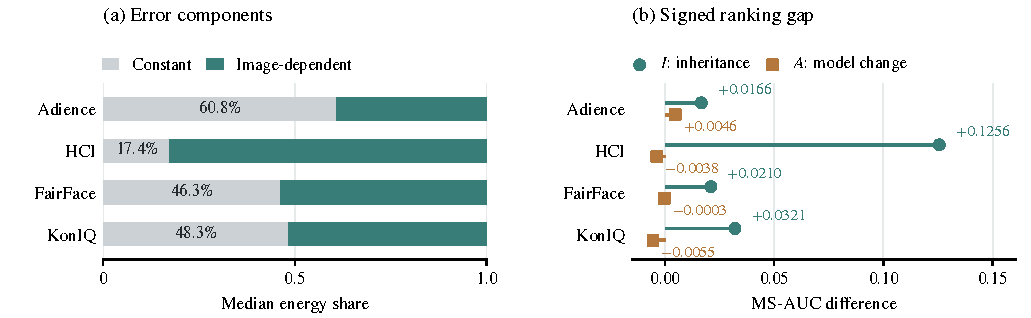
\includegraphics[width=\textwidth]{figures/supp/supp_b_error_diagnostic.pdf}
\caption{\textbf{Inheritance error and the remaining ranking gap.}
(a) Per-dataset median constant-component energy fraction $\kappa$; the complement is the image-dependent share.
(b) Mean signed MS-AUC differences $I$ and $A$ from Eq.~\eqref{eq:supp_fullsupport_gaps}, over the six missing-grade patterns and three seeds, equally averaged over nine adapter configurations.
Negative values indicate that the second score construction ranks better.
These are point summaries; a missing endpoint paired with its nearest seen anchor contributes $A=0$ by construction.}
\label{fig:supp_error_diagnostic}
\end{figure*}

To examine inheritance itself, we use the budget-matched full-support reference, FullSup.
Its displacement is $D^{\mathrm{FS}}=S^{\mathrm{FS}}-T$.
Applying the same inheritance rule gives the diagnostic scores $S^{\mathrm{FS\text{-}TIE}}=T+\mathcal L_{\mathcal U}(D^{\mathrm{FS}})$, denoted FS--TIE.
Define $e_m=D_m^{\mathrm{FS}}-[\mathcal L_{\mathcal U}(D^{\mathrm{FS}})]_m$.
The FullSup and FS--TIE margins against any seen grade differ by exactly $e_m$.
For an isolated interior grade, Proposition~4 of the main paper gives
$e_m=-\tfrac12(D_{m-1}^{\mathrm{FS}}-2D_m^{\mathrm{FS}}+D_{m+1}^{\mathrm{FS}})$.
The error is therefore proportional to the local curvature of adaptation along the grade axis.
Within an interior missing block, equal-weight error also contains a term from the grade's offset from the anchor midpoint; distance weights interpolate linear displacement exactly.

\noindent\textbf{Which part of the error can change the order?}
For a fixed missing--seen pair $(m,n)$, let $\mathbb E_{mn}$ average over test images whose true grades are $m$ or $n$.
We split the error into its mean $c_{mn}=\mathbb E_{mn}[e_m]$ and centered residual $r_{mn}(x)=e_m(x)-c_{mn}$:
\begin{equation}
\begin{aligned}
\mathbb E_{mn}[e_m^2]
&=c_{mn}^2+\mathbb E_{mn}[r_{mn}^2],\\
\kappa_{mn}
&=\frac{c_{mn}^2}{\mathbb E_{mn}[e_m^2]}.
\end{aligned}
\label{eq:supp_error_components}
\end{equation}
Here $\kappa_{mn}$ is the constant-component energy fraction for nonzero error.
For any two images, $e_m(x)-e_m(x')=r_{mn}(x)-r_{mn}(x')$: the constant cancels.
Only the image-dependent component can reorder images.
The diagnostic mean $c_{mn}$ describes this decomposition; it is separate from the validation-selected calibration offset $c^*$.

Figure~\ref{fig:supp_error_diagnostic}a quantifies the distinction.
The median constant-error share ranges from 17\% to 61\% across datasets.
A substantial part of displacement reconstruction error therefore leaves ranking unchanged.
The remaining residual can improve or worsen ranking according to how it changes pair margins.
Reconstruction error alone cannot determine the direction of the ranking change.

\noindent\textbf{Separating inheritance from changes in the adapted model.}
Let $R(Z)$ denote MS-AUC computed from scores $Z$ on the same test images and missing--seen pairs.
With $S^{\mathrm{TIE}}$ from the missing-grade adaptation run, define
\begin{equation}
\begin{aligned}
I
&=R(S^{\mathrm{FS}})
 -R(S^{\mathrm{FS\text{-}TIE}}),\\
A
&=R(S^{\mathrm{FS\text{-}TIE}})
 -R(S^{\mathrm{TIE}}).
\end{aligned}
\label{eq:supp_fullsupport_gaps}
\end{equation}
The total FullSup--TIE gap is exactly $I+A$.
The first term changes only the inherited coordinates within the FullSup model.
The second captures the change in anchors and seen scores between full-support and missing-grade adaptation.
Figure~\ref{fig:supp_error_diagnostic}b reports both signed terms.
For a missing endpoint and its nearest seen anchor, both inherited constructions recover the same zero-shot margin, forcing $A=0$.
Across dataset means, the inheritance term is larger in magnitude than the model-change term.
On HCI, the two terms are 0.126 and $-0.004$, respectively: most of the remaining mean FullSup--TIE gap lies in inheritance within the full-support model.
Proposition~4 characterizes this error, and Proposition~1 identifies the component that can change ranking.

\section{Grade Support and Missing-Grade Structure}
\label{sec:supp_grade_support}

We examine how ordinal transfer changes as target grades receive direct supervision and as the location of missing grades varies. A budget-matched full-support model provides a reference for the adaptation recovered through inheritance.

\subsection{From Missing to Partially Observed Grades}
\label{sec:supp_support_levels}

TIE supplies adaptation to grades without direct training support.

We use three support levels, 0\%, 10\%, and 20\%, under two protocols. The fixed-total protocol keeps the adaptation budget at 256 images while changing the target-grade support. The fixed-seen protocol retains the same seen-grade training images as target-grade support is added. These protocols give complementary views of supervision availability; their exact sample allocations are specified in Sec.~F.3.

Figure~\ref{fig:supp_support_levels} reports the MS-AUC gain of TIE over Adapted. The study covers CoOp-style, OrdinalCLIP-style, and Tip-Adapter-F (CE). Adience and HCI are evaluated under both protocols; FairFace and KonIQ use the fixed-total protocol.

\begin{figure*}[t]
\centering
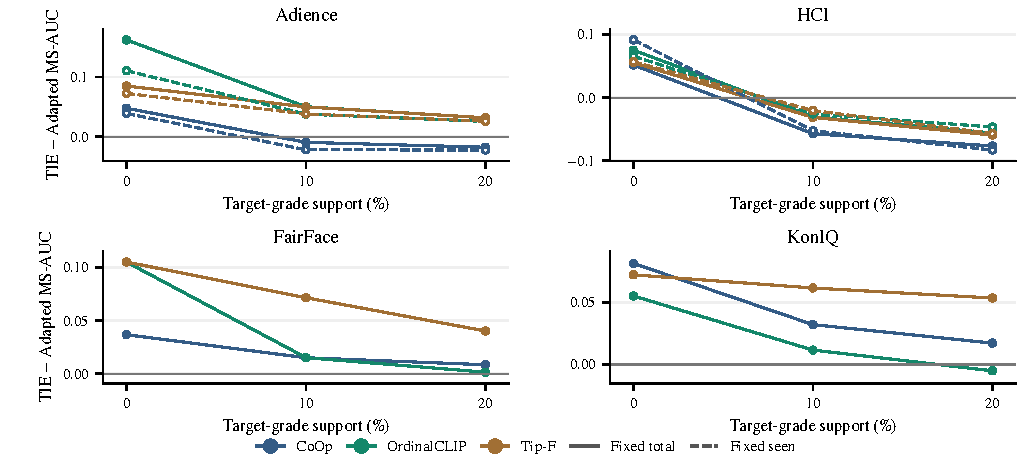
\includegraphics[width=\textwidth]{figures/supp/supp_c_support_levels.pdf}
\caption{\textbf{Sensitivity to grade-specific supervision.}
Change in MS-AUC from Adapted to TIE at 0\%, 10\%, and 20\% target-grade support. Colors distinguish the three adapter configurations. Solid lines use a fixed total training budget; dashed lines retain fixed seen-grade training images. Adience and HCI include both protocols, while FairFace and KonIQ use the fixed-total protocol. Each point is the mean under its corresponding protocol.}
\label{fig:supp_support_levels}
\end{figure*}

All 18 adapter--dataset--protocol trajectories show decreasing average ranking gains from 0\% to 10\% to 20\% support. The largest gains occur when target grades have no images of their own. Once direct supervision is introduced, inheritance contributes less additional information.

On HCI, TIE lowers MS-AUC for all three configurations at 10\% and 20\% target-grade support. Direct supervision reduces the need for inherited displacement, and the benefit of transfer depends on how much a grade has learned from its own images.

\subsection{Endpoints, Interior Grades, and Missing Blocks}
\label{sec:supp_missing_structure}

The main experiments use six missing-grade patterns. Table~\ref{tab:supp_missing_masks} gives their exact grade indices. The notation follows the main paper's one-based grade numbering. Three patterns omit interior grades; the other three involve the label-space endpoints.

\begin{table}[t]
\centering
\caption{\textbf{Missing-grade patterns.}
Grade indices are one-based. HCI and KonIQ share the same $K=5$ masks.}
\label{tab:supp_missing_masks}
\footnotesize
\setlength{\tabcolsep}{3pt}
\begin{tabular*}{\columnwidth}{@{\extracolsep{\fill}}lccc@{}}
\toprule
Pattern & Adience & FairFace & HCI/KonIQ \\
\midrule
Low endpoint & $\{1\}$ & $\{1\}$ & $\{1\}$ \\
Middle & $\{4\}$ & $\{5\}$ & $\{3\}$ \\
High endpoint & $\{8\}$ & $\{9\}$ & $\{5\}$ \\
Adjacent pair & $\{4,5\}$ & $\{4,5\}$ & $\{2,3\}$ \\
Separated pair & $\{2,7\}$ & $\{2,8\}$ & $\{2,4\}$ \\
Both endpoints & $\{1,8\}$ & $\{1,9\}$ & $\{1,5\}$ \\
\bottomrule
\end{tabular*}
\end{table}

\noindent\textbf{Endpoint restoration.}
For a missing endpoint $m$ and its nearest seen grade $n$, TIE copies $D_n$ and exactly recovers the zero-shot margin $T_m-T_n$. This property addresses a measurable adaptation loss. On endpoint patterns, Adapted falls below the zero-shot MS-AUC by 0.065, 0.028, 0.058, and 0.056 on Adience, HCI, FairFace, and KonIQ, respectively. TIE restores the reference ranking for the endpoint--neighbor comparisons.

\noindent\textbf{Interior transfer.}
With seen grades on both sides, inheritance retains information from their adapted displacements. At the original adaptation strength, TIE exceeds zero-shot interior MS-AUC by 0.113 on HCI, 0.025 on FairFace, and 0.096 on KonIQ. Thus, endpoint inheritance restores a reference margin, while interior inheritance can improve upon it.

For consecutive missing grades, equal-weight inheritance gives every grade in the block the same displacement. Their pairwise displacement difference cancels, recovering the zero-shot order within the block. Distance-weighted inheritance instead preserves changes across the anchor interval. Section~\ref{sec:supp_inheritance_rules} analyzes this distinction.

\subsection{Full-Support Reference}
\label{sec:supp_fullsupport}

We compare masked adaptation with FullSup, a budget-matched reference trained with labeled images from every grade. FullSup uses 256 training images and 64 validation images in total, distributed across the complete grade space. The masked models use the same budgets, with training and validation images drawn from seen grades.

FullSup provides a direct-supervision reference for missing-grade performance (Table~2(a) of the main paper). TIE closes 44--58\% of the Missing MAE gap on Adience, HCI, and FairFace. On KonIQ, TIE closes more than the full gap (111\%): its Missing MAE is below FullSup's for eight of nine configurations.

Gap closure is computed within each adapter before averaging, so it can differ slightly from the ratio of the mean errors in main-paper Table~2(a).

Across adapters, the MS-AUC gap-closure ratio has a median of 63\%. One setting is excluded because its FullSup improvement does not meet the reporting criterion in Sec.~\ref{sec:supp_f_metrics}.

\section{Generality across Adaptation Regimes and Domains}
\label{sec:supp_generality}

TIE operates on aligned zero-shot and adapted scores, rather than adapter parameters. We examine the same score-space rule under ordinal and knowledge-preserving adaptation, full fine-tuning, alternative pretrained backbones, and two additional grading domains. Each extension is evaluated within its own training and validation protocol.

\subsection{Ordinal and Knowledge-Preserving Adaptation}
\label{sec:supp_ordinal_adaptation}

Ordinal prompt learning already uses the structure of the grade space. Yet learning ordered prompts does not directly supervise the missing grades. In the main adapter matrix, TIE raises MS-AUC for OrdinalCLIP-style adaptation by 0.162 on Adience and 0.105 on FairFace. Ordinal representation learning and ordinal displacement transfer address different parts of adaptation.

\begin{table}[!t]
\centering
\caption{\textbf{Knowledge preservation and ordinal transfer.}
Formula-matched KgCoOp under two interior masks and three seeds. The first two columns report uncalibrated KgCoOp minus CoOp. The third is TIE minus KgCoOp MS-AUC. The final column is the independently calibrated TIE minus KgCoOp Missing MAE. Positive MAE differences indicate larger errors. All differences are computed before rounding.}
\label{tab:supp_kgcoop}
\footnotesize
\setlength{\tabcolsep}{2pt}
\begin{tabular*}{\columnwidth}{@{\extracolsep{\fill}}lrrrr@{}}
\toprule
& \multicolumn{2}{c}{KgCoOp $-$ CoOp}
& \multicolumn{2}{c}{TIE $-$ KgCoOp} \\
\cmidrule(lr){2-3}
\cmidrule(l){4-5}
Dataset
& $\Delta$AUC
& $\Delta$Miss.
& $\Delta$AUC
& $\Delta$Miss.$_{\mathrm{Cal}}$ \\
\midrule
Adience
& $+0.011$ & $+0.045$ & $+0.030$ & $+0.067$ \\
HCI
& $\mathbf{-0.118}$ & $\mathbf{-0.074}$
& $+0.157$ & $+0.017$ \\
FairFace
& $-0.004$ & $-0.001$
& $+0.045$ & $+0.214$ \\
KonIQ
& $-0.005$ & $-0.013$
& $+0.055$ & $-0.109$ \\
\bottomrule
\end{tabular*}
\end{table}

\begin{table*}[!t]
\centering
\caption{\textbf{Transfer beyond the primary adapter matrix.}
TIE minus Adapted, both before calibration, within each extension protocol. $\Delta$AUC denotes MS-AUC; negative MAE differences indicate improvement.
(a) Alternative pretraining, backbones, and SCUT facial-beauty prediction. (b) DDR severity grading; all nine backbone--adapter settings are shown. DDR values retain four decimal places to preserve the original small differences. Results from different protocols are not pooled.}
\label{tab:supp_extension_results}

\begin{minipage}[t]{0.48\textwidth}
\centering
\textbf{(a) Pretraining, backbones, and SCUT}\par
\smallskip
\footnotesize
\setlength{\tabcolsep}{2pt}
\begin{tabular*}{\linewidth}{@{\extracolsep{\fill}}llrr@{}}
\toprule
Setting & Adapter
& $\Delta$AUC$\uparrow$
& $\Delta$Miss.$\downarrow$ \\
\midrule
LAION / Adience & CoOp & $+0.032$ & $-0.511$ \\
LAION / Adience & OrdinalCLIP & $+0.122$ & $-0.747$ \\
LAION / HCI & CoOp & $+0.043$ & $-0.189$ \\
LAION / HCI & OrdinalCLIP & $+0.077$ & $-0.360$ \\
\midrule
RN50 / HCI & CoOp & $+0.071$ & $-0.237$ \\
RN50 / HCI & OrdinalCLIP & $+0.056$ & $-0.283$ \\
RN50 / HCI & Tip-F & $+0.033$ & $-0.266$ \\
\midrule
SCUT-FBP5500 & CoOp & $+0.120$ & $-0.059$ \\
SCUT-FBP5500 & OrdinalCLIP & $+0.188$ & $-0.083$ \\
\bottomrule
\end{tabular*}
\end{minipage}
\hfill
\begin{minipage}[t]{0.48\textwidth}
\centering
\textbf{(b) DDR: three backbones and adapters}\par
\smallskip
\footnotesize
\setlength{\tabcolsep}{1.6pt}
\begin{tabular*}{\linewidth}{@{\extracolsep{\fill}}llrrrr@{}}
\toprule
Backbone & Adapter
& $\Delta$AUC
& $\Delta$Miss.
& $\Delta$Seen
& $\Delta$All \\
\midrule
ViT-B/16 & CoOp
& $-0.0201$ & $-0.2900$ & $+0.2281$ & $+0.0061$ \\
ViT-B/16 & OrdinalCLIP
& $-0.0263$ & $-0.3045$ & $+0.2642$ & $+0.0191$ \\
ViT-B/16 & Tip-F
& $-0.0255$ & $-0.2905$ & $+0.2331$ & $+0.0072$ \\
\midrule
RN50 & CoOp
& $+0.0070$ & $-0.0455$ & $+0.0053$ & $-0.0163$ \\
RN50 & OrdinalCLIP
& $+0.0215$ & $-0.0825$ & $+0.0221$ & $-0.0287$ \\
RN50 & Tip-F
& $-0.0109$ & $-0.0454$ & $+0.0089$ & $-0.0149$ \\
\midrule
ViT-L/14 & CoOp
& $-0.0358$ & $-0.0687$ & $+0.0190$ & $-0.0205$ \\
ViT-L/14 & OrdinalCLIP
& $-0.0394$ & $-0.0885$ & $+0.0268$ & $-0.0291$ \\
ViT-L/14 & Tip-F
& $-0.0310$ & $-0.0686$ & $+0.0249$ & $-0.0187$ \\
\bottomrule
\end{tabular*}
\end{minipage}
\end{table*}

Knowledge-preserving adaptation provides another comparison. We evaluate a formula-matched KgCoOp implementation~\cite{yao2023kgcoop} with cosine regularization toward hand-crafted text embeddings. This control uses two interior missing-grade masks and three seeds per benchmark. It is distinct from the KgCoOp-style configuration in the main adapter matrix.

Table~\ref{tab:supp_kgcoop} shows a striking result on HCI: KgCoOp reduces Missing MAE relative to CoOp by 0.074, while MS-AUC falls by 0.118. Preserving pretrained knowledge does not necessarily preserve the missing--seen order. Applying TIE to KgCoOp raises MS-AUC on all four tasks, by 0.030--0.157.

The classification results reveal a second distinction. Before calibration, TIE also lowers KgCoOp's Missing MAE on all four tasks. After independent validation calibration, its Missing MAE is higher on Adience, HCI, and FairFace, but lower on KonIQ. FairFace shows the largest reversal: ranking improves by 0.045 while calibrated Missing MAE increases by 0.214. Ordinal transfer changes ranking; calibration determines how that ranking enters full-$K$ decisions.



A separate NumCLIP~\cite{du2024numclip} HCI experiment provides an interface-level comparison. Its adapted model predicts no missing-grade images in all 18 evaluated conditions. The ported implementation does not provide an aligned zero-shot score reference for the required $S=T+D$ construction, so it is not used as a TIE comparison.



\subsection{Full Fine-Tuning}
\label{sec:supp_full_finetuning}

We next examine full fine-tuning of the visual encoder and classification head. Unlike prompt-only adaptation, full fine-tuning changes the visual representation itself. The missing--seen ranking gain from TIE is $-0.0058$ on Adience, $+0.0077$ on HCI, $+0.0098$ on FairFace, and $+0.1987$ on KonIQ.

These results show that the value of transfer depends on the adapted score structure. Full fine-tuning can already improve missing--seen ranking even when missing-grade recall is low. TIE further improves ranking on three benchmarks, but not Adience. With calibration, TIE reduces Missing MAE relative to the simple binary-score control on all four tasks, while Adapted+C remains better on Adience and FairFace. Ranking recovery and calibrated classification performance remain distinct.

\subsection{Pretraining Sources and Backbones}
\label{sec:supp_pretraining_backbones}

Table~\ref{tab:supp_extension_results}a extends the comparison to LAION-pretrained CLIP~\cite{cherti2023reproducible} and a ResNet-50 backbone. With LAION weights, TIE improves MS-AUC in all four adapter--dataset settings and reduces Missing MAE in all four. On HCI with RN50, the three tested adapters also gain MS-AUC and lower Missing MAE.

The larger ViT-L/14 experiments provide a complementary adaptation diagnostic. Their adapted MS-AUC reaches 0.944, 0.815, 0.808, and 0.596 on Adience, HCI, FairFace, and KonIQ, respectively. Missing-grade recall nevertheless remains zero on HCI and KonIQ. Stronger adapted ranking alone does not guarantee that missing grades are selected by the full classifier.

These experiments span different adaptation contracts. The comparisons in Table~\ref{tab:supp_extension_results} are therefore performed within each protocol, rather than averaged across pretrained sources or backbones.

\subsection{Additional Domains}
\label{sec:supp_additional_domains}

We evaluate facial-beauty prediction on SCUT-FBP5500~\cite{liang2018scut} using its five official folds. TIE improves MS-AUC by 0.120 with CoOp-style adaptation and 0.188 with OrdinalCLIP-style adaptation. Missing MAE also decreases for both, by 0.059 and 0.083. These results extend displacement transfer to another subjective visual ordinal task.

We further evaluate five-grade diabetic-retinopathy severity on DDR~\cite{li2019ddr}. Table~\ref{tab:supp_extension_results}b reports all nine combinations of three CLIP backbones and three adapters. TIE reduces Missing MAE in every combination, while Seen MAE increases in every combination. MS-AUC improves in two of nine settings, and Overall MAE decreases in six. The medical extension thus shows a different balance between missing-grade recovery and ranking.

DDR uses a content-proxy-group split because patient identifiers are unavailable. The result demonstrates transfer behavior on a medical ordinal task without claiming patient-level independent validation.

Across these extensions, the same score-space operation can be applied after different forms of adaptation. Its effects on ranking and full-$K$ error depend on the learned displacement and the surrounding class competition. This is why the paper evaluates order and calibrated decisions separately.

\section{Derivations and Inference Algorithm}
\label{sec:supp_derivations}

We give the derivations behind the four propositions in the main paper and a single inference procedure. Throughout, $T$ denotes aligned zero-shot scores, $S$ the adapted scores, and $D=S-T$.

\subsection{Calibration and the Blending Family}
\label{sec:supp_calibration_proofs}

\noindent\textbf{Proposition 1: ranking invariance.}
For a fixed grade pair $(m,n)$ and scores $Z$, let $g^Z_{mn}(x)=Z_m(x)-Z_n(x)$.
A common positive scale $a$ and image-independent class biases $b$ give
\begin{equation}
 g^{aZ+b}_{mn}(x)=a\,g^Z_{mn}(x)+b_m-b_n.
 \label{eq:supp_affine_margin}
\end{equation}
This is strictly increasing in the original margin. Every comparison between two images, including ties, is preserved, and so is pair AUROC. The missing-grade bias $c$ is the special case $b_k=c\mathbf1[k\in\mathcal U]$.

\noindent\textbf{Proposition 2: the blending family.}
With $B_\lambda=T+\lambda D$ and $\Delta T_{mn}=T_m-T_n$, $\Delta D_{mn}=D_m-D_n$, calibration after blending produces
\begin{equation}
 g^{aB_\lambda+b}_{mn}
 =a(\Delta T_{mn}+\lambda\Delta D_{mn})+b_m-b_n.
 \label{eq:supp_blend_margin}
\end{equation}
Thus, for a fixed pair, calibration does not add rankings to the path indexed by $\lambda$. The reference is $\lambda=0$, and the adapted model is $\lambda=1$.

\subsection{Properties of the Inheritance Operator}
\label{sec:supp_operator_proofs}

Let $\mathcal Y=\{1,\ldots,K\}$ and fix a missing set $\mathcal U$ with a nonempty set of seen anchors $\mathcal O=\mathcal Y\setminus\mathcal U$. For each missing grade $m$, let $\ell(m)$ and $r(m)$ be its nearest seen grades below and above it, when available; $n(m)$ denotes the sole available anchor. Let $w_{mj}$ be $1/2$ on its two nearest bracketing seen grades, or $1$ on its sole available seen anchor, and zero otherwise. Then $\sum_{j\in\mathcal O}w_{mj}=1$ and
\begin{equation}
[\mathcal L_{\mathcal U}(D)]_k=
\begin{cases}
 D_k,&k\in\mathcal O,\\
 \sum_{j\in\mathcal O}w_{kj}D_j,&k\in\mathcal U.
\end{cases}
\label{eq:supp_operator_linear}
\end{equation}

\noindent\textbf{Proposition 3: structural properties.}
The first branch gives $S_k^{\mathrm{TIE}}=S_k$ for seen $k$. At a missing endpoint $m$ with nearest seen grade $n$, the sole weight is $w_{mn}=1$, hence
$g^{S^{\mathrm{TIE}}}_{mn}=(T_m+D_n)-(T_n+D_n)=g^T_{mn}$.
The weights are fixed by the grade mask, so $\mathcal L_{\mathcal U}$ is linear and $\mathcal L_{\mathcal U}(\lambda D)=\lambda\mathcal L_{\mathcal U}(D)$. These identities prove seen-score preservation, endpoint margin recovery, and commutation with global blending. A subsequent constant class bias retains the endpoint's pairwise ranking.

\noindent\textbf{Proposition 4: inheritance error.}
Consider the FullSup displacement $D^{\mathrm{FS}}$ at an interior grade $m$ with seen neighbors $m-1$ and $m+1$. Suppressing the image argument, its error after inheritance is
\begin{equation}
 e_m=-\tfrac12\bigl(D^{\mathrm{FS}}_{m-1}-2D^{\mathrm{FS}}_m+D^{\mathrm{FS}}_{m+1}\bigr).
 \label{eq:supp_curvature_proof}
\end{equation}
For every seen $n$, the FullSup and FS--TIE $m$--$n$ margins differ by exactly $e_m(x)$, since the seen-grade score is unchanged. If $e_m$ is constant across images, the difference is a class-pair offset and leaves ranking unchanged by Proposition 1. Section~\ref{sec:supp_inheritance_error} measures the constant and image-dependent components.

\subsection{Inference Algorithm and Cost}
\label{sec:supp_inference}

The grade mask determines all anchors before inference. The bias $c^*$ is selected once from seen-grade validation images under the main paper's common error budget; its candidate grid and selection rule are specified in Sec.~F.4. For a test image, the complete score operation is:

\noindent\textbf{TIE inference.}
\begin{algorithmic}[1]
 \Require Scores $T(x),S(x)$; mask $\mathcal U$; offset $c^*$
 \State $D\gets S(x)-T(x)$; $Z\gets S(x)$
 \For{$m\in\mathcal U$}
  \If{both $\ell(m)$ and $r(m)$ exist}
   \State $Z_m\gets T_m(x)+\tfrac12(D_{\ell(m)}+D_{r(m)})$
  \Else
   \State $Z_m\gets T_m(x)+D_{n(m)}$ (sole anchor)
  \EndIf
 \EndFor
 \State \Return $\displaystyle\arg\max_{k\in\mathcal Y}\{Z_k+c^*\mathbf1[k\in\mathcal U]\}$
\end{algorithmic}

The anchor map takes $O(K)$ preprocessing time. Computing $D$, inheriting all missing coordinates, and selecting the final grade each take $O(K)$ time per image and $O(K)$ score storage. These costs exclude obtaining $T$ and $S$ from the encoders. TIE introduces no trainable parameters.

\section{Experimental Protocols and Reproducibility}
\label{sec:supp_protocols}


\subsection{Datasets, Labels, and Prompts}
\label{sec:supp_data_prompts}

\begin{table}[!ht]
\centering
\caption{\textbf{Exact language interfaces.}
Templates and grade strings are reproduced verbatim.
Semicolons separate grade strings and are not inserted into the prompts.}
\label{tab:supp_f_prompts}
\begingroup
\fontsize{8}{9.5}\selectfont
\setlength{\tabcolsep}{3pt}
\renewcommand{\arraystretch}{1}
\begin{tabularx}{\columnwidth}{
  @{}
  >{\raggedright\arraybackslash}p{0.21\columnwidth}
  >{\raggedright\arraybackslash}X
  @{}
}
\toprule
Task & Language interface\\
\midrule
Adience & \texttt{a photo of a person aged \{grade\} years.} & \texttt{0 to 2}, \texttt{4 to 6}, \texttt{8 to 12}, \texttt{15 to 20}, \texttt{25 to 32}, \texttt{38 to 43}, \texttt{48 to 53}, \texttt{60 to 100} \\
HCI & \texttt{a historical color photograph taken in the \{grade\}.} & \texttt{1930s}, \texttt{1940s}, \texttt{1950s}, \texttt{1960s}, \texttt{1970s} \\
FairFace & \texttt{a photo of a person aged \{grade\} years.} & \texttt{0 to 2}, \texttt{3 to 9}, \texttt{10 to 19}, \texttt{20 to 29}, \texttt{30 to 39}, \texttt{40 to 49}, \texttt{50 to 59}, \texttt{60 to 69}, \texttt{more than 70} \\
KonIQ & \texttt{a photograph with \{grade\} image quality.} & \texttt{bad}, \texttt{poor}, \texttt{fair}, \texttt{good}, \texttt{excellent} \\
SCUT-FBP5500 & \texttt{a photo of a face with beauty score \{grade\} out of five.} & \texttt{one}, \texttt{two}, \texttt{three}, \texttt{four}, \texttt{five} \\
DDR & \texttt{a retinal fundus photograph showing \{grade\}.} & \texttt{no diabetic retinopathy}, \texttt{mild non-proliferative diabetic retinopathy}, \texttt{moderate non-proliferative diabetic retinopathy}, \texttt{severe non-proliferative diabetic retinopathy}, \texttt{proliferative diabetic retinopathy} \\
\bottomrule

\end{tabularx}
\endgroup
\end{table}

\begin{table*}[!t]
\centering
\caption{\textbf{Nine adapter configurations.}
Trainable components, score constructions, objectives, and optimization.
CE denotes cross-entropy; SORD uses the soft targets defined in Sec.~\ref{sec:supp_adapters}.
All unspecified base CLIP parameters remain frozen.}
\label{tab:supp_f_adapters}
\begingroup
\fontsize{8}{9.5}\selectfont
\setlength{\tabcolsep}{4pt}
\renewcommand{\arraystretch}{1}
\begin{tabularx}{\textwidth}{
  @{}
  >{\raggedright\arraybackslash}p{0.15\textwidth}
  >{\raggedright\arraybackslash}p{0.36\textwidth}
  >{\raggedright\arraybackslash}X
  @{}
}
\toprule
Configuration & Components, scores, and objective & Optimization and selection\\
\midrule
CoOp-style &
Shared four-token context initialized with \texttt{a photo of a}; fixed lexical ranks.
$S_k=100f^\top p_k$; CE. &
SGD, learning rate 0.002, momentum 0.9, weight decay 0.
Cosine schedule for 100 epochs.
Select minimum NLL at epochs 50 and 100; earlier checkpoint on ties.\\
\addlinespace[2pt]

OrdinalCLIP-style &
Learned context and three base rank tokens, one token per base rank; linear rank interpolation~\cite{li2022ordinalclip}.
$S_k=100f^\top p_k$.
CE plus text-to-image KL divergence with equal weights. &
Adam, learning rate $10^{-4}$, weight decay 0, 50 epochs.
Multiply learning rate by 0.1 at epoch 30 for age tasks, and at epochs 25 and 35 for HCI/KonIQ.
Select minimum NLL over epochs; earlier checkpoint on ties.\\
\addlinespace[2pt]

KgCoOp-style &
CoOp components and score.
Objective:
$\mathrm{CE}+\frac{8}{K}\sum_{k=1}^{K}\|p_k-p_k^0\|_2^2$,
using all $K$ normalized text features. &
Same SGD, cosine schedule, checkpoint candidates, and selection rule as CoOp-style.\\
\addlinespace[2pt]

TaskRes-style (CE) &
Only a zero-initialized $K\times512$ prototype residual $\Delta W$ is trained.
$S=100\operatorname{norm}(P+0.5\Delta W)f$.
CE. &
Adam with learning rate in $\{0.0002,0.002\}$, $\epsilon=10^{-8}$, weight decay 0.
Cosine schedule, maximum 60 epochs; first-epoch learning rate $10^{-5}$; patience 10.
Select minimum NLL across epochs and learning rates, retaining the earlier candidate on exact ties.\\
\addlinespace[2pt]

TaskRes-style (SORD) &
Same prototype residual and score as TaskRes-style (CE); SORD supervision. &
Same optimization and selection as TaskRes-style (CE).\\
\addlinespace[2pt]

Tip-Adapter-F (CE) &
Unconstrained support keys $W$, initialized with unit image features; fixed one-hot values $V$.
$S=T+\alpha V^\top\exp[-\beta(\mathbf1-Wf)]$.
The exponential is elementwise; CE. &
AdamW with learning rate in $\{10^{-4},10^{-3}\}$, $\epsilon=10^{-4}$, weight decay 0.01.
Cosine schedule, maximum 60 epochs; patience 10.
Fit at $\alpha=1$, $\beta=5.5$.
Retain the minimum-NLL epoch per learning rate, then select learning rate,
$\alpha\in\{0.1,1,10\}$, and
$\beta\in\{1,2,5.5\}$ jointly by NLL.
Exact ties follow ascending learning-rate/$\alpha$/$\beta$ order.\\
\addlinespace[2pt]

Tip-Adapter-F (SORD) &
Same keys, values, and score as Tip-Adapter-F (CE); SORD supervision. &
Same optimization, checkpoint selection, and parameter grids as Tip-Adapter-F (CE).\\
\addlinespace[2pt]

M3 &
Rank-8 LoRA on the final visual attention QKV and output weights, plus a $512\to128\to K$ GELU residual head.
$S_k=100z_\theta^\top p_k^0+h_k$.
The head input is centered and scaled using the native training mean and RMS.
CE.
$T$ uses the unadapted image encoder. &
AdamW with visual learning rate $10^{-4}$ and head learning rate $10^{-3}$; weight decay $10^{-3}$.
Maximum 60 epochs; patience 10.
Select minimum NLL; earlier checkpoint on ties.\\
\addlinespace[2pt]

TEXT\_ONLY &
An independent visual LoRA fit with the same visual construction as M3.
The residual head is disabled and frozen; $S_k=100z_\theta^\top p_k^0$, distinct from frozen $T$; CE. &
AdamW, learning rate $10^{-4}$, weight decay $10^{-3}$.
Maximum 60 epochs; patience 10.
Select minimum NLL; earlier checkpoint on ties.\\
\bottomrule

\end{tabularx}

\medskip
\begin{minipage}{\textwidth}
\noindent\textit{Prompt initialization.}
CoOp-style and KgCoOp-style use the suffixes \texttt{person aged \{grade\} years} for age, \texttt{\{grade\}} for HCI, and \texttt{\{grade\} image quality} for KonIQ.
OrdinalCLIP-style uses the task-specific initialization strings ``age estimation: the age of the person is'' for age tasks, ``historical dating: a photo taken in the'' for HCI, and ``aesthetics assessment: the quality of the photo is'' for KonIQ.
\end{minipage}
\endgroup
\end{table*}

\begin{table}[!t]
\centering
\caption{\textbf{Target-grade support allocations.}
(a) Pre-mask quotas and per-target counts at 0/10/20\% support.
Fixed-total has 256 images on all four tasks.
(b) Fixed-seen totals on Adience and HCI.}
\label{tab:supp_f_support}
\begingroup
\fontsize{8}{9.5}\selectfont
\setlength{\tabcolsep}{3pt}
\renewcommand{\arraystretch}{1}
\textbf{(a) Pool quotas and target counts}\par
\smallskip
\begin{tabularx}{\columnwidth}{
  @{}
  >{\raggedright\arraybackslash}p{0.22\columnwidth}
  >{\raggedright\arraybackslash}X
  >{\centering\arraybackslash}p{0.22\columnwidth}
  @{}
}
\toprule
Task & Pool quota & 0/10/20\%\\
\midrule
Adience & 32 per grade & 0/4/7\\
HCI / KonIQ & 52 for grade 1; 51 otherwise & 0/6/11\\
FairFace & 29 for grades 1--4; 28 otherwise & 0/3/6\\
\bottomrule
\end{tabularx}

\medskip
\textbf{(b) Fixed-seen sample totals}\par
\smallskip
\begin{tabularx}{\columnwidth}{
  @{}
  >{\raggedright\arraybackslash}X
  r
  >{\centering\arraybackslash}p{0.36\columnwidth}
  @{}
}
\toprule
Task and target pattern & Seen & Total: 0/10/20\%\\
\midrule
Adience, one grade & 224 & 224/228/231\\
Adience, two grades & 192 & 192/200/206\\
HCI, low endpoint & 204 & 204/210/215\\
HCI, middle or high & 205 & 205/211/216\\
HCI, adjacent or separated pair & 154 & 154/166/176\\
HCI, both endpoints & 153 & 153/165/175\\
\bottomrule
\end{tabularx}

\endgroup
\end{table}

\begin{table}[!t]
\centering
\caption{\textbf{Validation-only selection.}
All selectors use the bias grid and error budget in Sec.~\ref{sec:supp_calibration_protocol}.
Blend strengths are $\lambda\in\{0,0.1,\ldots,1.5,2\}$.}
\label{tab:supp_f_selectors}
\begingroup
\fontsize{8}{9.5}\selectfont
\setlength{\tabcolsep}{3pt}
\renewcommand{\arraystretch}{1}
\begin{tabularx}{\columnwidth}{
  @{}
  >{\raggedright\arraybackslash}p{0.19\columnwidth}
  >{\raggedright\arraybackslash}X
  @{}
}
\toprule
Selector & Sequence and choice\\
\midrule
Class bias & For each condition let $q_i(Z)=\max_{k\in\mathcal O}Z_k(x_i)-\max_{k\in\mathcal U}Z_k(x_i)$ on seen validation. Using $Z\in\{S,S^{\mathrm{TIE}}\}$, set $c_{\min}=\lfloor\min q\rfloor-1$, $c_{\max}=\lceil\max q\rceil+1$. Candidates $\{-\infty\}\cup\{c_{\min},c_{\min}+1,\ldots,c_{\max}\}$. Largest feasible $c$ under uncalibrated Adapted nMAE$+0.005$ (numerical tolerance $10^{-15}$); each path chooses its own. $-\infty$ suppresses missing grades; empty feasible set is blocked. Full-$K$ argmax ties choose the lowest grade. \\
Blend-S & $\lambda\in\{0,0.1,\ldots,1.5,2\}$. First minimize uncalibrated seen-validation nMAE of $T+\lambda(S-T)$ within the same risk budget; largest $\lambda$ among exact minimum-risk ties. Then select its own largest feasible bias on the condition's frozen shared grid above. No feasible bias: blocked, no replacement offset. \\
Blend-A & Same $17$ strengths and condition-specific bias grid. Independently select the largest feasible bias for every $\lambda$; discard infeasible candidates. Minimize resulting calibrated seen-validation nMAE; largest $\lambda$ among exact equal-risk ties. If all candidates are infeasible, block the path. Test scores do not select either deployment strength. \\
Binary control & Its own unit-step grid uses the same floor/ceiling rule applied to its validation score switches alone, plus $-\infty$. Same uncalibrated Adapted budget and largest-feasible rule; a failed guard remains blocked. \\
\bottomrule

\end{tabularx}
\endgroup
\end{table}

The main benchmarks are Adience~\cite{eidinger2014age} ($K=8$), HCI~\cite{palermo2012dating} ($K=5$), FairFace~\cite{karkkainen2021fairface} ($K=9$), and KonIQ-10k~\cite{hosu2020koniq} ($K=5$).
Each image has one ordered grade and is evaluated against the full $K$-class label space.
Test sizes per seed are 4,377, 198--199, 14,356, and 2,010, respectively.

KonIQ grades are training-split MOS quintiles with cut points 2.7016, 3.1385, 3.4167, and 3.6400.
Table~\ref{tab:supp_f_prompts} gives the exact reference templates and ordered grade strings.
Learned-context and ordinal-prompt configurations retain the same grade identities as their zero-shot references.


\subsection{Adapter Configurations}
\label{sec:supp_adapters}

All nine main configurations use OpenAI CLIP ViT-B/16~\cite{radford2021clip} and produce aligned pre-softmax scores for the same grade vocabulary.
They cover learned context prompts~\cite{zhou2022coop}, ordinal rank prompts~\cite{li2022ordinalclip}, knowledge-preserving prompts~\cite{yao2023kgcoop}, prototype residuals~\cite{yu2023taskres}, and trainable cache adapters~\cite{zhang2022tipadapter}.


The CE and SORD configurations differ in their supervision targets.
SORD uses distance-based soft ordinal labels~\cite{diaz2019sord}, here
$q_j\propto\exp[-(j-y)^2/2]$ over all $K$ grades.
M3 combines visual low-rank adaptation (LoRA)~\cite{hu2022lora} with a residual head.
TEXT\_ONLY trains the visual LoRA independently with the residual head disabled and text embeddings frozen.
Its name refers to scoring with the frozen text prototypes alone, without M3's residual head.

In Table~\ref{tab:supp_f_adapters}, $f$ is the unit frozen-image feature, $p_k$ and $p_k^0$ are adapted and reference unit text features, and $P$ stacks reference text features as rows.
The adapted visual feature is $z_\theta$, and $h_k$ is the residual-head output for grade $k$.
The operator $\operatorname{norm}$ normalizes matrix rows.
For cache adapters, $W$ contains support keys and $V$ their one-hot grade values.

All configurations use batch size 32.
Checkpoint and hyperparameter selection use hard-label negative log-likelihood (NLL) on seen-grade validation images.
The main KgCoOp-style recipe differs from the formula-matched control in Sec.~\ref{sec:supp_ordinal_adaptation}.


\subsection{Missing Masks and Support Budgets}
\label{sec:supp_f_masks}

The six missing-grade masks are listed in Table~\ref{tab:supp_missing_masks}.
The main protocol uses seeds 101, 202, and 303, with 256 training and 64 validation images drawn only from seen grades.
Counts are balanced across the $K-|\mathcal U|$ seen grades, differing by at most one image.
Every test split retains all $K$ grades.
The main matrix therefore contains $9\times4\times6\times3=648$ conditions.

The support experiments start from a same-seed, balanced, 256-image training-only pool.
Let $n_k^{\mathrm{pool}}$ be the pre-mask quota of target grade $k$.
At support fraction $r$, its sample count is
$n_k(0)=0$ and
$n_k(r)=\max(1,\lceil r n_k^{\mathrm{pool}}\rceil)$ for $r>0$.
Thus, 10\% and 20\% refer to the target grade's pool quota.

Fixed-total keeps 256 images by removing seen-grade images in round-robin order as target images are added.
Its target and seen counts are
$\sum_{k\in\mathcal U}n_k(r)$ and
$256-\sum_{k\in\mathcal U}n_k(r)$.
Fixed-seen retains the exact seen-image IDs from the masked pool and adds target images, using its own matched 0\% baseline.
Both protocols use the six masks and three seeds above.
Table~\ref{tab:supp_f_support} gives all sample allocations.


\subsection{Scores, Calibration, and Blend Selection}
\label{sec:supp_calibration_protocol}

All score constructions use aligned grade indices and a common pre-softmax scale.
The displacement $D=S-T$ is computed before calibration.
Missing-grade calibration adds a class bias, following the calibrated-stacking formulation~\cite{chao2016gzsl}.
For scores $Z$, prediction uses
$\arg\max_k\{Z_k(x)+c_Z^*\mathbf1[k\in\mathcal U]\}$.

The validation budget uses normalized mean absolute error,
\begin{equation}
\operatorname{nMAE}_{\mathrm{seen}}(Z)
=
\frac{1}{N_{\mathrm{val}}(K-1)}
\sum_{i\in\mathrm{val}}
|\hat y_Z(x_i)-y_i|,
\label{eq:supp_f_nmae}
\end{equation}
where $N_{\mathrm{val}}$ is the number of seen-grade validation images.
A bias is feasible when
$\operatorname{nMAE}_{\mathrm{seen}}(Z+c\mathbf1_{\mathcal U})
\le
\operatorname{nMAE}_{\mathrm{seen}}(S)+0.005$,
with numerical tolerance $10^{-15}$.

For validation image $i$, define
$v_i(Z)=\max_{k\in\mathcal O}Z_k(x_i)-\max_{k\in\mathcal U}Z_k(x_i)$.
The shared condition-specific grid uses
$\mathcal V=\{v_i(S),v_i(S^{\mathrm{TIE}}):i\in\mathrm{val}\}$,
with
$c_{\min}=\lfloor\min\mathcal V\rfloor-1$,
$c_{\max}=\lceil\max\mathcal V\rceil+1$, and
$\mathcal C=\{-\infty\}\cup\{c_{\min},c_{\min}+1,\ldots,c_{\max}\}$.
Each path selects its own largest feasible bias.
An empty feasible set is reported as infeasible.
Full-$K$ argmax ties select the lowest grade.

Table~\ref{tab:supp_f_selectors} specifies the two Blend selectors.
Both use seen validation only.
The best Blend in Sec.~\ref{sec:supp_best_blend} is instead the retrospective test maximum on the 17-point grid.
FullSup retains the same total 256/64 training/validation budgets, distributed across all $K$ grades.


\subsection{Metrics, Aggregation, and Uncertainty}
\label{sec:supp_f_metrics}

For each adjacent missing--seen pair $(m,n)$, pair AUROC ranks images by $Z_m-Z_n$, using test images of those two true grades, with $m$ positive and ties counting one half.
MS-AUC is the arithmetic mean over these pairs.
It is computed from finite pre-calibration scores; the $-\infty$ candidate is used only to suppress missing-grade predictions.

Missing MAE first averages absolute grade error within each missing grade, then across missing grades.
Seen and Overall MAE average over their respective test images.
All MAEs are in grade units.

For the main adapter matrix, results first average over six masks and three seeds within each adapter--dataset setting, then equally over the nine configurations.
The interior analysis uses three masks.
Extension results use the masks, seeds, or folds stated in Sec.~\ref{sec:supp_generality}.

FullSup gap closure is computed within each adapter--dataset setting before aggregation.
A ratio is reported when the FullSup improvement over Adapted exceeds $10^{-8}$ and its original paired 95\% interval lies above zero.
The only excluded MS-AUC ratio is TaskRes-style (SORD) on Adience.

The ranking intervals in Fig.~\ref{fig:supp_config_curves} and Table~\ref{tab:supp_best_blend} use 10{,}000 paired group-bootstrap replicates with fixed checkpoints.
Both methods use the same resampled test groups.
Adience groups follow the supplied \texttt{user\_id} metadata; HCI, FairFace, and KonIQ use content-proxy groups.
These intervals are pointwise.

For DDR, content-proxy groups are used because patient identifiers are unavailable.

The counts 34/36 and 35/36 denote positive point estimates across adapter--dataset settings for all masks and interior masks, respectively, at the original strength.
The count 59/64 denotes nonzero dataset--strength comparisons whose paired pointwise 95\% intervals lie above zero.

\subsection{Figure Construction and Implementation}
\label{sec:supp_f_figures}

The main paper's Fig.~1 uses KonIQ, CoOp-style adaptation, seed 101, and a missing middle grade.
Grade 3 (\emph{fair}) is compared with seen grade 2 (\emph{poor}), using 411 and 401 test images.
Pair AUROC is computed from the original per-image score margins.
The displayed offsets are $c^*=6$ for Adapted and $c^*=0$ for TIE.

The main paper's Fig.~2 uses 81 interior-mask conditions per dataset and the 17-point strength grid, with paired bootstrap intervals for TIE minus Blend.
The margin-shift illustration in Fig.~1b is schematic.
The score-processing algorithm and its $O(K)$ cost are given in Sec.~\ref{sec:supp_inference}.

\bibliographystyle{ieeenat_fullname}
\bibliography{main}
\end{document}
